\documentclass[a4paper, 10pt]{scrartcl}
\usepackage[a4paper,top=2.9cm,bottom=2.9cm,left=2.7cm,right=2.7cm]{geometry}
\usepackage[utf8]{inputenc}
% PACCHETTO PER LA LINGUA
\usepackage[english]{babel}
% PACCHETTI PER EQUAZIONI E SIMBOLI MATEMATICI
\usepackage{amsmath}
\usepackage{amsfonts}
\usepackage{amssymb}
\usepackage{mathtools}
% PACCHETTI PER FIGURE, SUBFIGURE E FIGURE PLACEMENT
%\usepackage{wrapfig}
\usepackage{subcaption}
\usepackage{float}
% PACCHETTI PER CAPTION E TABELLE
\usepackage{caption}
\captionsetup{tableposition=bottom, figureposition=bottom, font=small}
\captionsetup[subfigure]{width=0.9\textwidth, format=hang}

% PACCHETTI PER GRAFICA E COLORI
\usepackage{graphicx}
\usepackage[dvipsnames]{xcolor}

% RIFERIMENTI IPERTESTUALI
\usepackage[colorlinks, citecolor=NavyBlue, linkcolor=blue, unicode]{hyperref}
%% autoref di equazioni con (numero)
\addto\extrasenglish{\def\equationautorefname~#1\null{(#1)\null}}
% PACCHETTI VARI E PERSONALIZZAZIONI
%\usepackage{mparhack}
%\usepackage{ragged2e}

% PACCHETTO PER BIBLIOGRAFIA
%\usepackage{natbib}
%\bibliographystyle{unsrt}
\usepackage[sorting=none]{biblatex}
\usepackage{csquotes}
\addbibresource{citations.bib}
\DeclareSourcemap{
  \maps[datatype=bibtex]{
    \map{
      % Remove language
      \step[fieldset=language, null]
    }
    \map{
      % If it contains a field eprinttype...
      \step[fieldsource=eprinttype, final]
      % ... remove the urldate and url
      \step[fieldset=urldate, null]
      \step[fieldset=url, null]
    }
    \map{
      % If it is not @online, always remove urldate and url
      \pernottype{online}
      % ... remove the urldate and url
      \step[fieldset=urldate, null]
      \step[fieldset=url, null]
    }
    \map{
      % If it is @online remove month, year, urldate
      \pertype{online}
      \step[fieldset=urldate, null]
      \step[fieldset=month, null]
      \step[fieldset=year, null]
    }
  }
}

\setlength\parindent{0pt}

\title{\LARGE{Report of first year activities}}
\author{\large{PhD student: Dario Zarcone}\\\large{Supervisor: Prof. Salvatore Miccichè}}
\date{\normalsize{October 21st, 2024}}
\subject{\small{Università degli Studi di Palermo\\Dipartimento di Fisica e Chimica - Emilio Segrè\\PhD Course in Physical and Chemical Sciences\\Cycle XXXIX}}

\begin{document}
\maketitle

This report summarizes the activities and projects I undertook during the first year of my PhD in Physical Sciences at the University of Palermo. My work spanned both academic research and educational initiatives.

The main research project involved a collaboration with the Prosecutor's Office of Palermo, where we studied historical data on homicides in Sicily. Additionally, we developed tools to extract information from legal documents at scale, including the implementation of a full-text search engine.

In a similar effort to gain insights through the lens of complex systems, we built a network of people and companies connected to mafia-related individuals.

I also participated in educational projects with high schools, such as the PNLS (Piano Nazionale Lauree Scientifiche) in statistical physics, organized by Prof. Miccichè, and the Coding Girls project, which promotes gender equality in STEM fields.

The following sections detail these projects, concluding with a list of the courses, schools, and other activities I attended or contributed to.

\section{Analysis of Murders in Sicily}

In collaboration with the Prosecutor's Office of Palermo, I worked on a project that focused on the study of data concerning murders, attempted murders and disappearances in Sicily. This dataset is particularly valuable, as it includes all known murders and disappearances that occurred during the First and Second Mafia Wars, as well as the Maxi Trial period and the subsequent so-called "stragista" (massacre) period, sometimes referred to as the Third Mafia War. Each record in the dataset includes the date and location of the murder.

The data is heterogeneous and, in some cases, incomplete. As a result, a thorough data cleaning operation was necessary to extract usable information. Despite these challenges, we successfully performed an analysis on the time series and spatial distribution of the events.

For the temporal analysis, we explored potential analogies with earthquake dynamics. Specifically, in seismology, aftershocks follow a power-law decay described by the Omori law:
\begin{equation}
  n(t) = \frac{k}{(t+c)^p}
\end{equation}
where \(n(t)\) is the number of aftershocks at time \(t\), and \(k\), \(c\), and \(p\) are parameters. This kind of dynamics is present also in other types of complex systems, for example in financial market \cite{lillo_power-law_2003}. Interestingly, the dynamics of murders in Sicily seem to have a "foreshocks" dynamics (\autoref{fig:omicidi}), like an inverse Omori law. Additionally, we found that the inter-event times (i.e., the time intervals between consecutive murders) are distributed according to a power-law (\autoref{fig:intertimes}), similarly to what happens in earthquakes \cite{lippiello_scaling_2012}.

By grouping murders that occurred within one week of each other, we could classify these events into "\textit{avalanches}", and the sizes of these avalanches also appear to follow a power-law distribution. This analysis also draws a parallel to another complex system, the brain: in this case, the avalanches are \textit{neuronal avalanches}, and display a power-law behaviour in their size and duration distribution \cite{lombardi_temporal_2014}.

\begin{figure}[H]
  \centering
  \begin{subfigure}[t]{.55\textwidth}
    \centering
    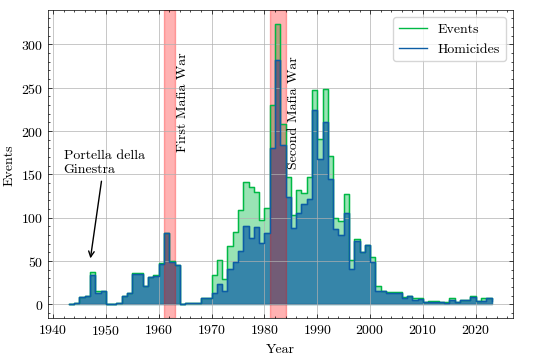
\includegraphics[width=\textwidth]{figures/omicidi.png}
    \caption{Monthly distribution of events in the dataset, with annotations highlighting significant periods. Each time, the number of violent events rises to a peak and then abruptly drops off.}
    \label{fig:omicidi}
  \end{subfigure}%
  \begin{subfigure}[t]{.36\textwidth}
    \centering
    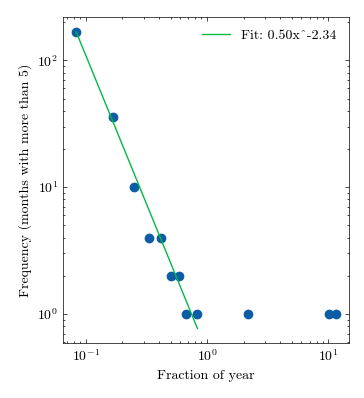
\includegraphics[width=\textwidth, trim={0 0.6cm 0 0},clip]{figures/intertimes.png}
    \caption{Log-log plot of inter-event times (with precision of months), only for months with more than 5 homicides. The distribution is a power-law.}
    \label{fig:intertimes}
  \end{subfigure}
  \caption{Examples of time analysis of the murders dataset.}
\end{figure}


For the spatial analysis, we utilized the Google Maps API to localize the murders in space. Although the dataset is incomplete, we focused initially on homicides that occurred in Palermo. Using this geolocation information, we developed an interactive map of homicides in the city (\autoref{fig:interactivemap}) and created a choropleth map displaying the distribution of murders across Palermo's 25 neighborhoods.
By comparing these murder densities to historical population data from each neighborhood, we identified areas that were over-represented or under-represented in terms of homicide frequency compared to a null hypothesis based on population distribution (\autoref{fig:overunder}).

\begin{figure}[h]
  \centering
  \begin{subfigure}[t]{.41\textwidth}
    \centering
    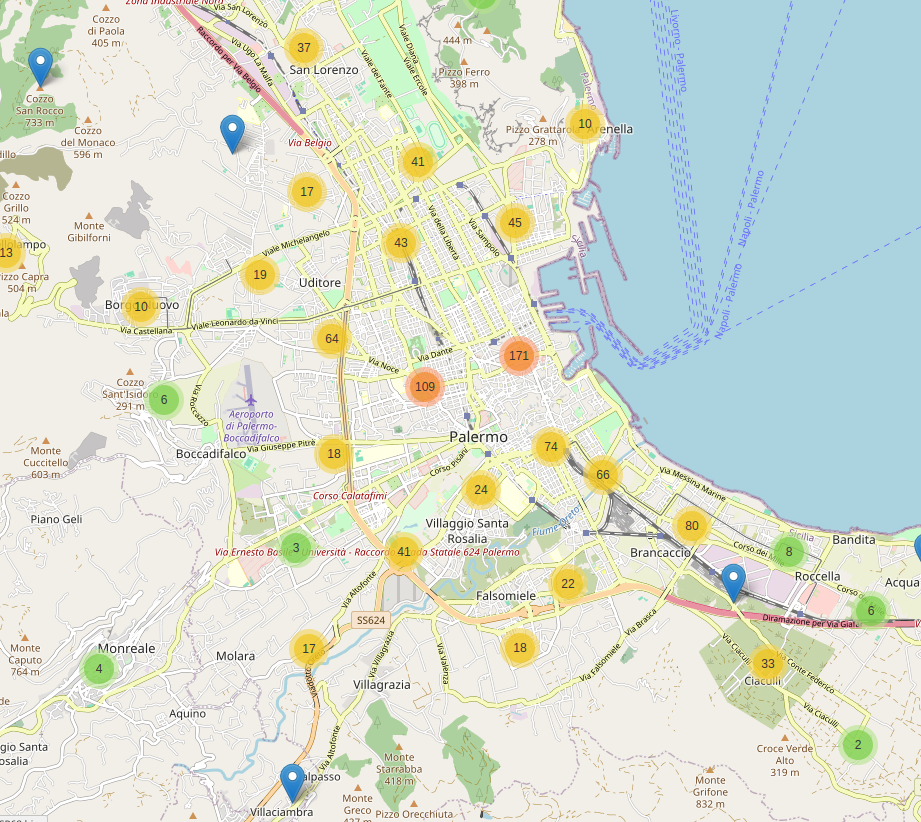
\includegraphics[width=\textwidth]{figures/interactivemap.png}
    \caption{Screenshot of the interactive map of murders in the Palermo area. Each point represents a cluster of homicides. By zooming in, more detailed information becomes available.}
    \label{fig:interactivemap}
  \end{subfigure}%
  \begin{subfigure}[t]{.41\textwidth}
    \centering
    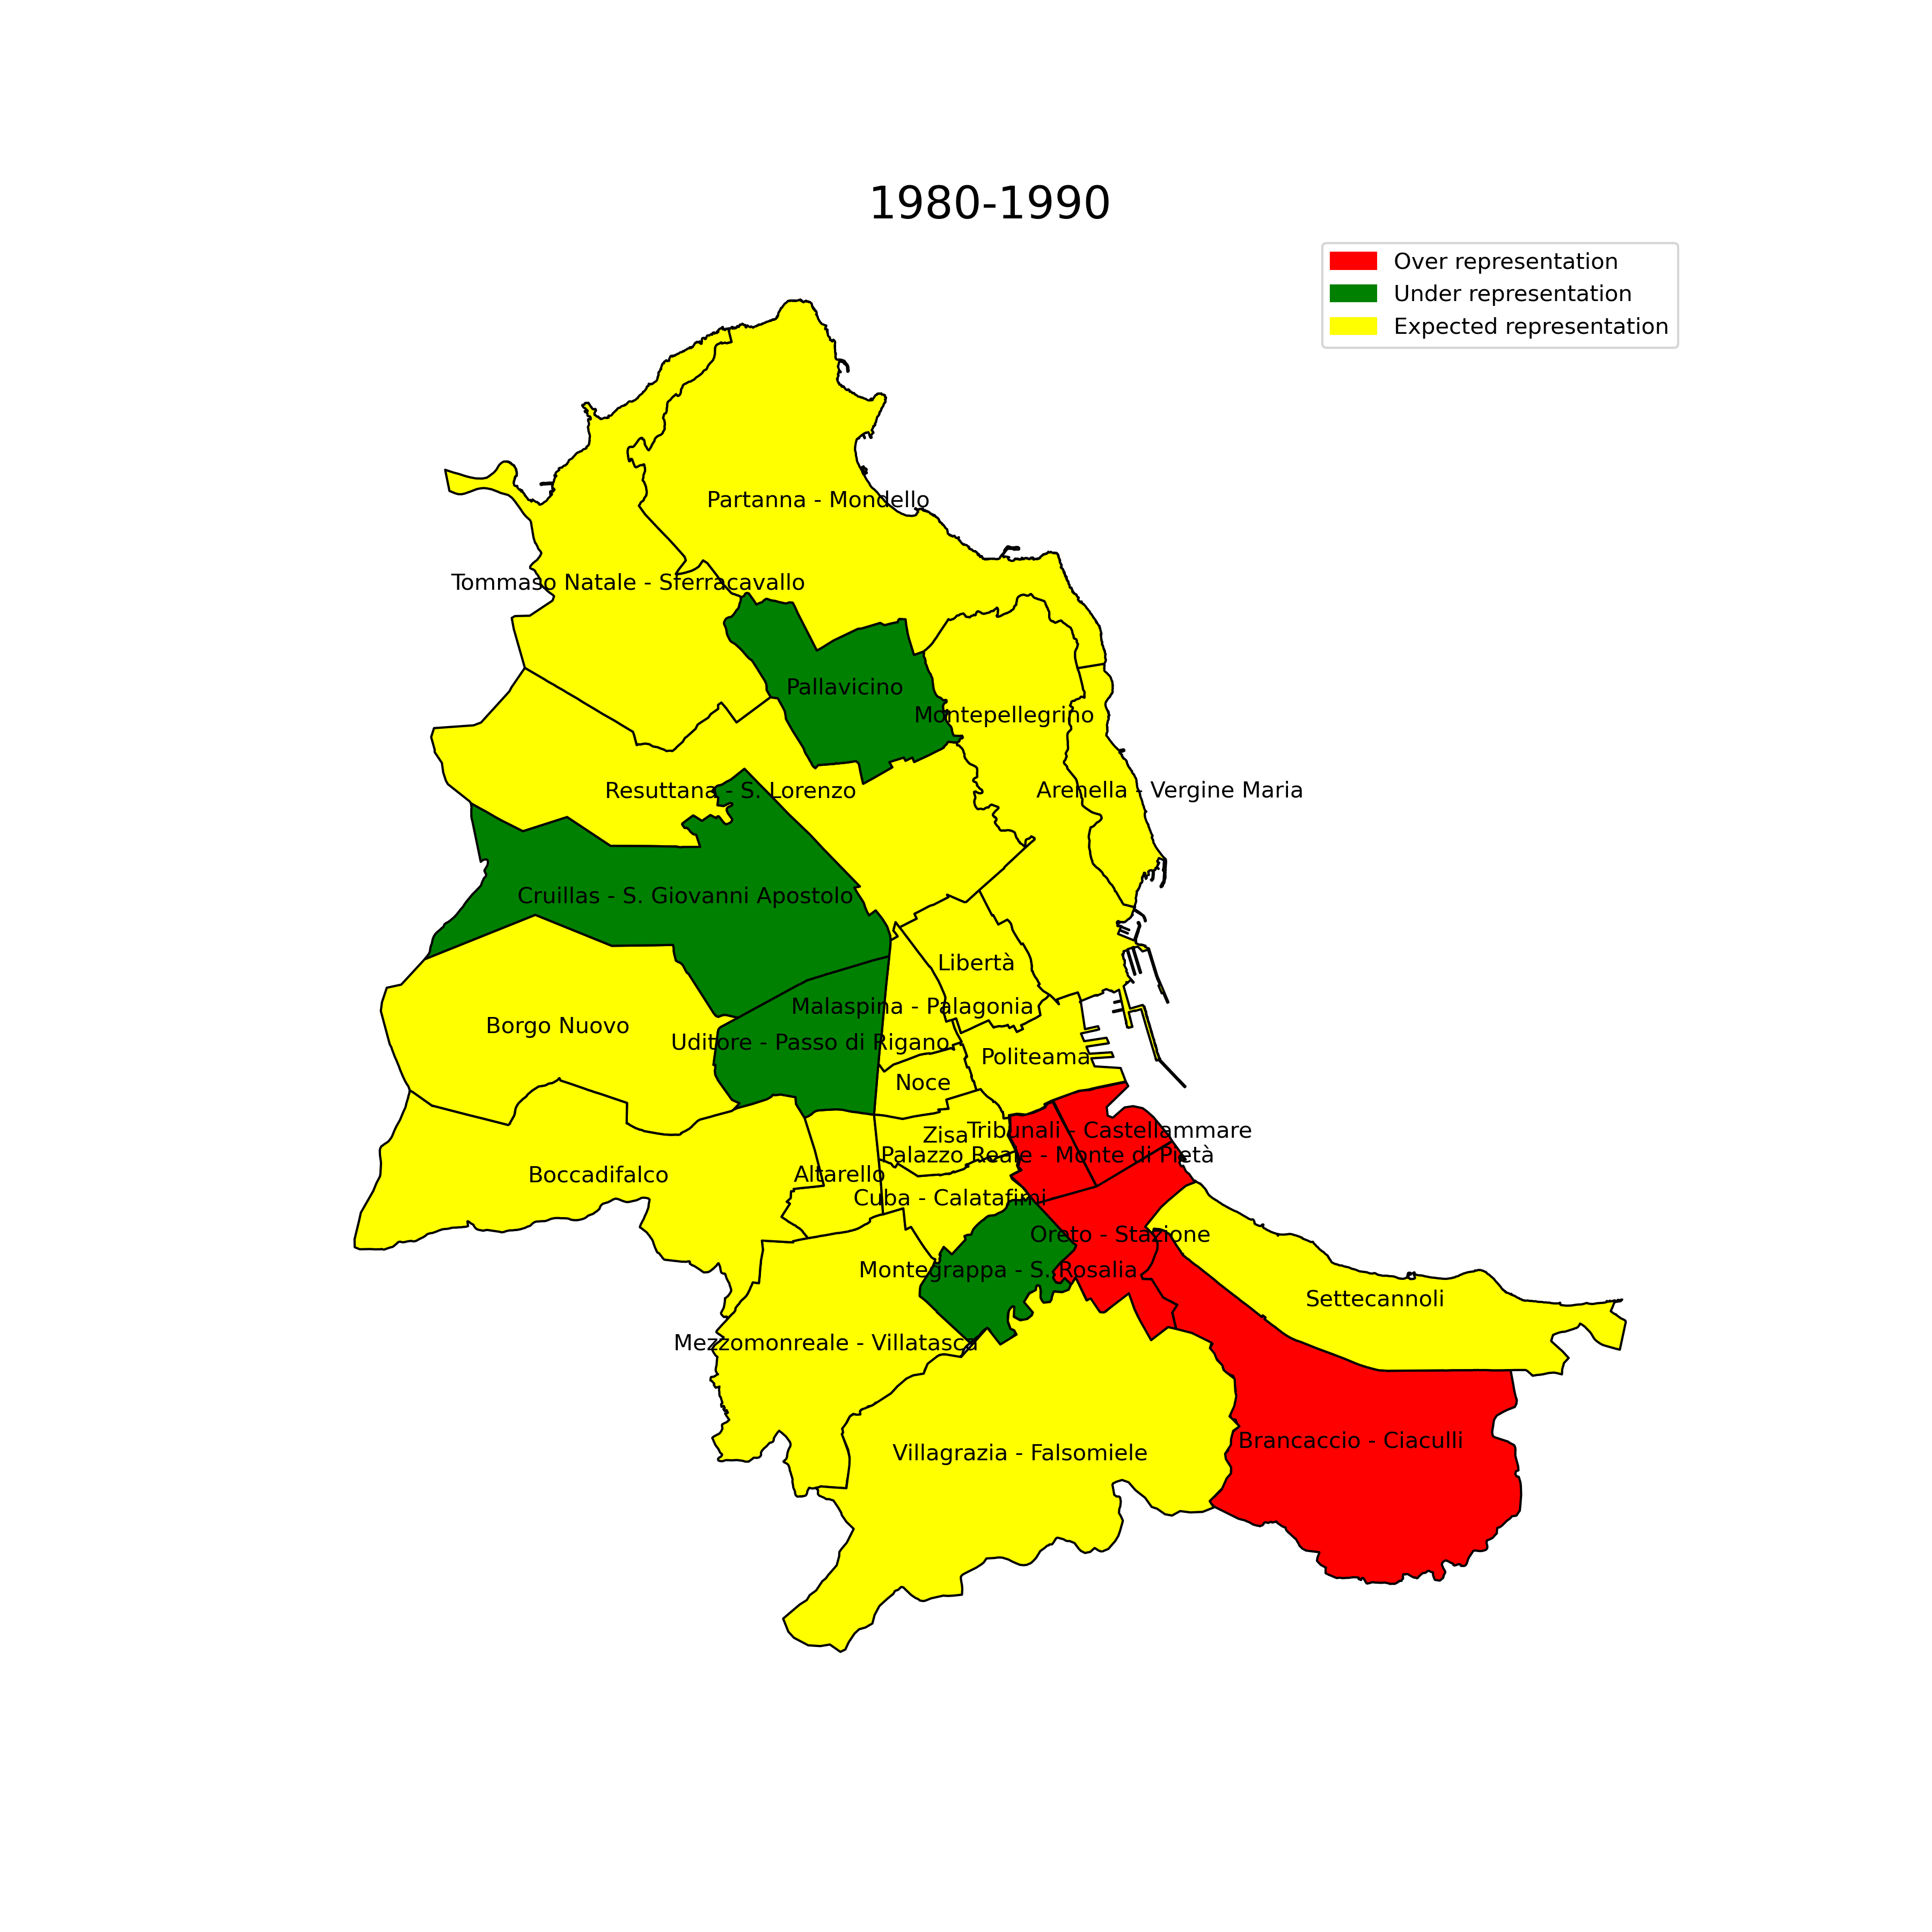
\includegraphics[width=\textwidth]{figures/palermomap-1980.png}
    \caption{Over- and under-representation of murders in Palermo's neighborhoods, relative to population, during the period of the Second Mafia War (1980-1990).}
    \label{fig:overunder}
  \end{subfigure}
  \caption{Examples of spatial analysis of the murders dataset.}
\end{figure}


Although we have not yet developed a complete model to explain our findings, the data exhibits similarities to that of earthquake occurrences or brain signals — events localized in time and space, which occur in bursts. The correlation structures are non-trivial and are a focus of study within the field of complex systems. To deepen our understanding, I, along with Prof. Miccichè, met with Prof. Eugenio Lippiello and Prof. Lucilla De Arcangelis at the Physics Department of Vanvitelli University in Caserta. They are experts in applying complex systems methods to the study of earthquakes and brain signals, and they provided us with valuable insights on how to approach the analysis of this data.

\section{Implementation of a Full-Text Search Engine for Legal Documents}

Another interesting dataset owned by the Prosecutor's Office of Palermo consists of legal documents, like trial sentences and procedural documents, of trials related to Cosa Nostra. These documents are often very long - sometimes thousands of pages — and the information within them is often scattered and difficult to extract systematically. A detailed analysis of such documents might provide valuable insights into relationships between individuals, locations and events. For instance, if two individuals appear together in a legal sentence, it is likely that they are connected, either through personal relations, shared actions, or in some other way. Similarly, if two individuals appear in documents related to the same trial, they likely have some form of connection.

Although we had no access to such valuable database, nevertheless we designed, in collaboration with the Prosecutor's Office, a tool for automatic \textit{information retrieval} from the corpus of documents. We implemented the tool on the set of documents already considered in \cite{tumminello_anagraphical_2021}.

In particular, we explored natural language processing (NLP) techniques that could identify names of people and places. However, performing such extraction at scale, across millions of pages, is a difficult computational challenge. For this reason, we decided to implement a full-text search engine capable of handling large-scale document collections \cite{baeza-yates_modern_2011}.

The core of our implementation is based on Elasticsearch \cite{noauthor_elasticsearch:_nodate}, an open-source search engine that is widely used for handling large volumes of text data. Elasticsearch allows for fast and scalable retrieval of information using an \textit{inverted index} \cite{baeza-yates_modern_2011}: instead of storing the entire content of each document, an index is created that maps each unique \textit{term} to the documents in which it appears. This allows for efficient querying, even across large datasets, by quickly finding all documents that contain specific terms or combinations of terms.

Having in mind that the available documents might be in various formats, from plain text documents to Microsoft Office documents to scanned images of paper documents, we had to implement a \textit{preprocessing} pipeline to standardize the input. This pipeline ingests documents in different formats and feeds them to the search engine, applying optical character recognition (OCR) when needed to extract the text

The search engine also supports advanced queries, so we are able to look for relationships between entities like individuals or places mentioned in the same context. This is particularly interesting for our research, as the connections, studied with the tools of complex networks, may reveal patterns and relationships.

As of now, we have completed the implementation of the tool and we were able to train people in the Prosecutor's Office to the use of the search engine. This tool is expected to greatly enhance our ability to extract structured knowledge from unstructured legal texts.

\section{Building a Network of People and Companies}

As part of Spoke 8 of the GRINS Project \cite{noauthor_grins_nodate}, which funds a portion of our research and my PhD scholarship, we gained access to several databases related to Italian companies. Specifically, we have access to the AIDA database \cite{noauthor_aida_nodate}, the CRIBIS database \cite{noauthor_cribis:_nodate}, both containing information on Italian companies, and ContrattiPubblici \cite{noauthor_il_nodate}, a database on public procurements in Italy.

AIDA contains information about all active companies in Italy, including their addresses, financial statements, advisors, directors, and other relevant details. Using this database, we were able to extract data about companies linked to a list of individuals, particularly those involved in mafia-related activities who had been convicted of crimes associated with organized crime.

To explore the relationships between these individuals and companies, we employed a breadth-first search strategy. Starting from our initial list of mafia-related individuals ("seed"), we expanded the search by three degrees of separation, creating three "shells" of connections between people and companies. This allows us to capture not only direct links between individuals and companies but also indirect relationships (for example, individuals connected through a shared company).

The resulting dataset enabled us to construct a bipartite network, with one set of nodes representing individuals and the other representing companies. In this network, edges connect individuals to the companies with which they are associated, either as directors, advisors, or shareholders. By analyzing the topology of this network, we aim to identify potential risk indicators based on its structural properties. We are investigating the presence of a community structure (statistically validated communities), the presence of cliques and other topological features that may serve as indicators of heightened risk for illegal activities or further mafia-related connections.

Although our research is still in its early stages, we were able to model these relationships as a complex network. In future work, we plan to apply network science techniques to study the connectivity patterns in greater depth, with the goal of developing indicators based on network metrics which could help flagging suspicious clusters of companies or individuals for further investigation.

\section{Educational initiatives}
\subsection*{PNLS - Statistical Physics}
In the context of the National Plan for Scientific Degrees (PNLS) in Statistical Physics, organized by Prof. Miccichè at the University of Palermo, I had the opportunity to work with high school students, assisting the professor during lessons and developing interactive simulations of complex systems, so to help students grasp key concepts in statistical physics by allowing them to experiment and visualize how varying system parameters affect physical behavior.

One of the core simulations I developed was an interactive model of the \textit{logistic map}\footnote{The interactive logistic map I developed can be explored here: \url{https://chaos-visualization.streamlit.app/}}. The logistic map is a mathematical model used to describe population dynamics, defined by the equation:
\begin{equation}
  x_{n+1} = r x_n (1 - x_n)
\end{equation}
where \(x_n\) represents the population at time step \(n\), and \(r\) is a parameter that controls the growth rate. The logistic map is characterized by the presence of fixed points, periodic oscillations, and chaotic dynamics. By interacting with the model, students were able to observe how small changes in parameters can lead to dramatically different outcomes, making it an ideal tool for introducing concepts related to chaos theory.

Additionally, I developed an interactive simulation of percolation on a two-dimensional lattice\footnote{The interactive percolation simulation can be used here: \url{https://2dpercolation-visualization.streamlit.app/}}. Here students could manipulate the probability \(p\) that a site in the lattice is occupied, allowing them to explore the critical point at which a spanning cluster forms. This hands-on approach made it easier for students to visualize how systems behave near criticality.

To further engage the students I created a physical simulation of the Ising model on a 64x64 LED matrix, controlled by an Arduino-like board. The Ising model is a classic model in statistical mechanics used to study ferromagnetism, where each site on a lattice can be in one of two states (representing magnetic spins). The model demonstrates how macroscopic order can emerge from microscopic interactions. By physically interacting with the LED matrix, students could change the temperature and observe how spin alignment changes, facilitating a deeper understanding of phase transitions.

Providing students with interactive and physical tools to explore these concepts helped bridge the gap between abstract theory and tangible understanding. By engaging with simulations and physically manipulating the systems, students were able to internalize complex ideas such as chaos, critical phenomena, and phase transitions, thus fostering a deeper interest in the study of statistical physics.

\subsection*{Coding Girls Project}

The Coding Girls project, by Fondazione Mondo Digitale \cite{noauthor_coding_2022}, is a national initiative aimed at promoting gender equality and inclusion in STEM fields, with a particular focus on coding. The project is active in over 30 Italian cities, including Palermo, where it operates in collaboration with the University of Palermo.

As part of this initiative, I was responsible for training over twenty physics students in the use of Arduino. These students, in turn, went to various high schools across Palermo, where they prepared high school students for a final Hackathon event. During the Arduino training sessions, the focus was on hands-on activities, so that they could have the necessary skills to mentor high schoolers.

Additionally, I conducted a Python course at Liceo Scientifico Galileo Galilei in Palermo. In a series of three lectures, I taught the basics of the Python programming language, using real-world examples to make the content more engaging and relatable. Around twenty high school students participated in this course, learning essential programming concepts such as variables, loops, and functions. Following the course, these students took part in the "Coding with Python" section of the Hackathon, where I assisted them in developing a project on the theme of climate change.

\section{Courses, Conferences, Schools, and Other Activities}

\subsection*{Courses}
\subsubsection*{PhD Courses}
\begin{itemize}
  \item \textbf{Project Management in the Scientific-Spatial Context} - Prof. Giuseppina Micela - 20 hours (with exam): My group and I developed a project for an Arduino School aimed at physics students and high schoolers, using all the project management tools we learned.
  \item \textbf{Introduction to Agent-Based Models} - Prof. Salvatore Miccichè - 20 hours (with exam): I developed a fully interactive generalization of the Ising model to analyze the similarities between the Schelling model and the Ising model.
  \item \textbf{Open Quantum Systems and Quantum Machine Learning} - Prof. Salvatore Lorenzo and Prof. Luca Innocenti - 20 hours
\end{itemize}

\subsubsection*{Other Courses}
\begin{itemize}
  \item \textbf{Econophysics} - Prof. Rosario Mantegna - 20 hours: Course for the PhD in "Complex Systems for Physical, Socio-economic, and Life Sciences" at the University of Catania.
  \item \textbf{Artificial Intelligence and Deep Learning} - Prof. Giosué Lo Bosco - 48 hours: Course for the Master Degree in "Data, Algorithms and Machine Intelligence" at the Dipartimento di Matematica e Informatica, University of Palermo.
  \item \textbf{Information Retrieval and Natural Language Processing} - Prof. Giovanni Pilato - 48 hours: Course for the Master Degree in "Data, Algorithms and Machine Intelligence" at the Dipartimento di Matematica e Informatica, University of Palermo.
\end{itemize}

\subsection*{Conferences}
\begin{itemize}
  \item \textbf{Statistics and Data Science 2024 (SDS 2024)} - Palermo, April 11th-12th, 2024
  \item \textbf{VIII Conference of Italian Physics Students (CISF24)} - Turin, April 17th-21st, 2024: I delivered an oral presentation titled "Nascosto in piena vista: Il fenomeno mafioso come esempio modello di sistema complesso."
\end{itemize}

\subsection*{Schools}
\begin{itemize}
  \item \textbf{School of the Italian Society of Statistical Physics (SIFS School 2024)} - Catania, August 26th - September 5th, 2024
\end{itemize}

\subsection*{Other Activities}
\begin{itemize}
  \item Participation in the \textbf{European Researchers' Night} - Palermo, September 27th, 2024
\end{itemize}

%\bibliography{citations}
\printbibliography

\end{document}
